Anomaly detection is the process of detecting patterns in a given data set that
do not conform to an ``expected'' behavior \cite{Chandola:2007}, although it is
often difficult to accurate predict expected patterns and distributions for data
sets. The terms `anomaly' and `outlier' are used synonymously, both within this
thesis and more generally in the field of statistics.

According to \citeauthor{Hawkins:1980} \cite{Hawkins:1980}:
\begin{quote}
An outlier is an observation which deviates so much from the other observations
as to arouse suspicions that it was generated by a different mechanism.
\end{quote}

Anomaly and outlier detection are challenging areas that have gained much
interest within the field of computer science. The importance of anomaly
detection is due to the fact that anomalies in data translate to significant
(and often critical) actionable information in a wide variety of application
domains \cite{Chandola:2007}. Over time, many techniques for anomaly detection
have been developed for specific application domains, as well as more generic
techniques \cite{Chandola:2007}.

%%%%%%%%%%%%%%%%%%%%%%%%%%%%%%%%%%%%%%%%%%%%%%%%%
% What are Anomalies?
%%%%%%%%%%%%%%%%%%%%%%%%%%%%%%%%%%%%%%%%%%%%%%%%%
\subsection{What are Anomalies?}
\label{anomalyDetection:whatAre}
Anomalies are patterns in data that do not conform to a well defined notion of
normal behavior. \autoref{fig:2d-anomalies} illustrates anomalies in a simple
2-dimensional data set. The data has two normal regions, $N_1$ and $N_2$, since
most observations lie in these two regions. Points that are sufficiently far
away from the regions, such as points $o_1$ and $o_2$, and points in region
$O_3$, are considered to be anomalies.

\begin{figure}
    \centering
    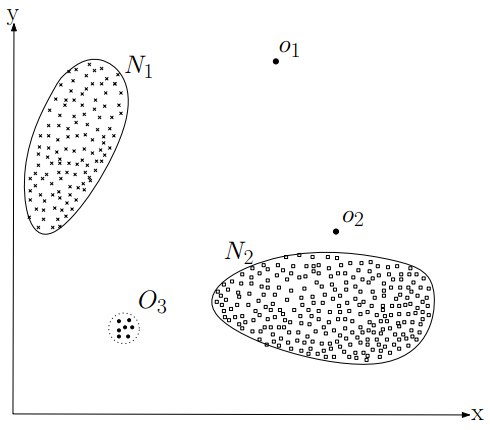
\includegraphics[width=0.5\textwidth]{anomalies/2d}
    \caption[A simple example of anomalies in a 2-dimensional data set.]
        {A simple example of anomalies in a 2-dimensional data set
        \cite{Chandola:2007}.}
    \label{fig:2d-anomalies}
\end{figure}

%%%%%%%%%%%%%%%%%%%%%%%%%%%%%%%%%%%%%%%%%%%%%%%%%
% Challenges
%%%%%%%%%%%%%%%%%%%%%%%%%%%%%%%%%%%%%%%%%%%%%%%%%
\subsection{Challenges}
\label{anomalyDetection:challenges}
A straightforward anomaly detection approach, is to define a region representing
`normal' behaviour and declare any observation in the data which does not belong
to this normal region as an anomaly. But several factors make this apparently
simple approach very challenging:

\begin{itemize}

\item Defining a normal region which encompasses every possible normal behaviour
is very difficult. In addition, the boundary between normal and anomalous
behaviour is often not precise. Thus an anomalous observation which lies close
to the boundary can actually be normal, and vice-versa.

\item When anomalies are the result of malicious actions, the malicious
adversaries often adapt themselves to make the anomalous observations appear
like normal, thereby making the task of defining normal behavior more difficult.

\item In many domains normal behavior keeps evolving and a current notion of
normal behavior might not be sufficiently representative in the future.

\item The exact notion of an anomaly is different for different application
domains. For example, in the medical domain a small deviation from normal (for
example, fluctuations in body temperature) might be an anomaly, while similar
deviation in the stock market domain (for example, fluctuations in the value of
a stock) might be considered as normal. Thus applying a technique developed in
one domain to another is not straightforward.

\item Availability of labeled data for training/validation of models used by
anomaly detection techniques is usually a major issue.

\item Often the data contains noise which tends to be similar to the actual
anomalies and hence is difficult to distinguish and remove.

\end{itemize}

Due to the above challenges, the anomaly detection problem, in its most general
form, is not easy to solve. In fact, most of the existing anomaly detection
techniques solve a specific formulation of the problem. The formulation is
induced by various factors such as nature of the data, availability of labeled
data, type of anomalies to be detected, etc. Often, these factors are determined
by the application domain in which the anomalies need to be detected.

Researchers have adopted concepts from diverse disciplines such as statistics,
data mining, statistics, information theory and spectral theory in order to gain
an increased understanding of anomalies \cite{Chandola:2007}.

%%%%%%%%%%%%%%%%%%%%%%%%%%%%%%%%%%%%%%%%%%%%%%%%%
% Similar Problems
%%%%%%%%%%%%%%%%%%%%%%%%%%%%%%%%%%%%%%%%%%%%%%%%%
\subsection{Similar Problems}
\label{anomalyDetection:similarProblems}
Anomaly detection is an intentionally broad specifier for a class of
more-specific statisctical challenges. For example, whilst being distinct from,
anomaly detection is a similar problem (in terms of complexity and approach) to
that of \emph{noise removal} and \emph{noise accomodation}, both of which are
aimed at removing the effects of unwanted \emph{noise} in the data. Noise can be
defined as any data which is not of specific interest to the analyst, but in its
presence hinders data analysis techniques \cite{Chandola:2007}. It is often
critical to data analysis to remove or mitigate the effects that noise has to
the properties of the host data set.

In contrast, the problem of \emph{novelty detection} can often be impeded by
techniques that attempt to remove anomalous data from a data set. \emph{Novelty
detection} is process of discovering emerging patterns in a data set, to provide
an indication of the future state of a system. The distinction between novel
pattern and anomalies is that novel patterns are incorporated into the data
model after detection \cite{Chandola:2007}.

%%%%%%%%%%%%%%%%%%%%%%%%%%%%%%%%%%%%%%%%%%%%%%%%%
% Classification
%%%%%%%%%%%%%%%%%%%%%%%%%%%%%%%%%%%%%%%%%%%%%%%%%
\subsection{Classification}
\label{anomalyDetection:classification}
In general, two different kinds of outliers exist: \emph{global outliers} and 
\emph{local outliers}. Global outliers are distinct with respect to the whole
data set, while local outliers are distinct with respect to data points in their
local neighbourhood \cite{Vries:2011}. The task of global outlier detection has
undergone much research \citeNeeded, but this has not been the case for local
outlier detection. In the paper \citetitle{Vries:2011}, \citeauthor{Vries:2011}
optimises the use of \gls{LOF} (see \autoref{localOutlierFactor}) for large and
high-dimensional data and proposes projection-indexed nearest-neighbours --- a
novel technique that exploits extended nearest-neighbour sets in a
reduced-dimensional space --- to create an accurate approximation for
$k$-nearest-neighbour distances, which is used as the core density measurement
within \gls{LOF} \cite{Vries:2011}.

%%%%%%%%%%%%%%%%%%%%%%%%%%%%%%%%%%%%%%%%%%%%%%%%%
% Types of Anomalies
%%%%%%%%%%%%%%%%%%%%%%%%%%%%%%%%%%%%%%%%%%%%%%%%%
\subsection{Types of Anomalies}
\label{anomalyDetection:types}
Anomalies can be classified into three categories \cite{Chandola:2007}:

\begin{description}

\item[Point anomaly] If an individual data instance can be considered as
anomalous with respect to the rest of data, then the instance is termed as a
point anomaly. This is the simplest type of anomaly. Referring to
\autoref{fig:2d-anomalies}, points $o_1$ and $o_2$, as well as all points in
region $O_3$ lie outside the boundary of the normal regions, and are hence point
anomalies.

\item[Contextual anomalies] If a data instance is anomalous in a certain
context, but not otherwise, then it is termed a contextual anomaly. The notion
of a context is induced by the structure in the data set and has to be specified
as part of the problem formulation.

\begin{figure}
    \centering
    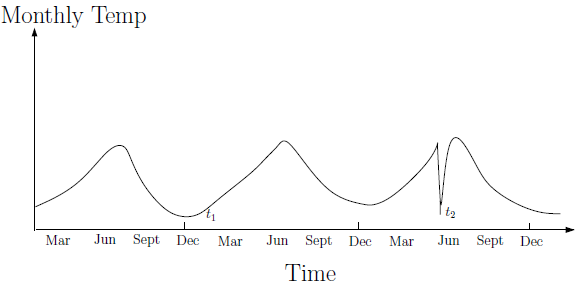
\includegraphics[width=0.5\textwidth]{anomalies/contextual}
    \caption[Contextual anomaly $t_2$ in a temperature time series.]
        {Contextual anomaly $t_2$ in a temperature time series. Note that the
        temperature at time $t_1$ is same as that at time $t_2$ but occurs in a
        different context and hence is not considered as an anomaly
        \cite{Chandola:2007}.}
    \label{fig:contextual-anomalies}
\end{figure}

Contextual anomalies have been most commonly explored in time-series data and
spatial data. \autoref{fig:contextual-anomalies} shows one such example for a
temperature time series which shows the monthly temperature of an area over last
few years. A temperature of $35^\circ F$ might be normal during the winter (at
time $t_1$) at that place, but the same value during summer (at time $t_2$)
would be an anomaly.

\item[Collective anomalies] If a collection of related data instances is
anomalous with respect to the entire data set, it is termed as a collective
anomaly. The individual data instances in a collective anomaly may not be
anomalies by themselves, but their occurrence together as a collection is
anomalous. \autoref{fig:collective-anomalies} illustrates an example which shows
a human electrocardiogram output. The highlighted region denotes an anomaly
because the same low value exists for an abnormally long time. Note that that
low value by itself is not an anomaly.

\begin{figure}
    \centering
    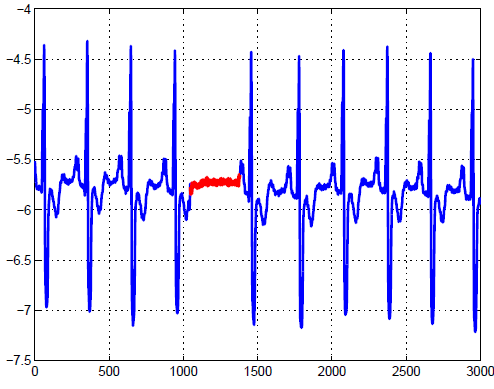
\includegraphics[width=0.5\textwidth]{anomalies/collective}
    \caption[Collective anomaly corresponding to an \emph{atrial premature
        contraction} in an human electrocardiogram output.]
        {Collective anomaly corresponding to an \emph{atrial premature
        contraction} in an human electrocardiogram output
        \cite{Goldberger:2000}.}
    \label{fig:collective-anomalies}
\end{figure}

\end{description}

%%%%%%%%%%%%%%%%%%%%%%%%%%%%%%%%%%%%%%%%%%%%%%%%%
% Distance Based
%%%%%%%%%%%%%%%%%%%%%%%%%%%%%%%%%%%%%%%%%%%%%%%%%
\subsection{Distance Based}
\label{anomalyDetection:approaches:distance}
In this approach, one looks at the local neighborhood of points for an example
typically defined by the $k$ nearest examples (also known as neighbours). If the
neighbouring points are relatively close, then the example is considered normal;
if the neighbouring points are far away, then the example is considered unusual.
The advantages of distance-based outliers are that no explicit distribution
needs to be defined to determine unusualness, and that it can be applied to any
feature space for which we can define a distance measure \cite{Bay:2003}.

Although distance is an effective non-parametric approach to detecting outliers,
the drawback is the amount of computation time required. Straightforward
algorithms, such as those based on nested loops, typically require $O(N^2)$
distance computations. This quadratic scaling means that it will be very
difficult to mine outliers as we tackle increasingly larger data sets. This is a
major problem for many real databases where there are often millions of records
\cite{Bay:2003}.

Researchers have tried a variety of approaches to find these outliers
efficiently. The simplest are those using nested loops \cite{Bay:2003}. In the
basic version one compares each example with every other example to determine
its $k$ nearest neighbors. Given the neighbors for each example in the data set,
simply select the top $n$ candidates according to the outlier definition. This
approach has quadratic complexity as we must make all pairwise distance
computations between examples.

Another method for finding outliers is to use a spatial indexing structure such
as a KD-tree, R-tree, or X-tree to find the nearest neighbors of each candidate
point. One queries the index structure for the closest $k$ points to each
example, and as before one simply selects the top candidates according to the
outlier definition. For low-dimensional data sets this approach can work
extremely well and potentially scales as $O(N \log N)$ if the index tree can
find an example's nearest neighbors in $\log N$ time. However, index structures
break down as the dimensionality increases \cite{Bay:2003}.

% Pruning Rule
\subsubsection{Pruning Rule}
\label{anomalyDetection:approaches:distance:pruning}
% TODO

%%%%%%%%%%%%%%%%%%%%%%%%%%%%%%%%%%%%%%%%%%%%%%%%%
% Distribution Based
%%%%%%%%%%%%%%%%%%%%%%%%%%%%%%%%%%%%%%%%%%%%%%%%%
\subsection{Distribution Based}
\label{anomalyDetection:approaches:distribution}
A common distribution considered when modelling data is the `Normal'
distribution. Using this model, the probability that a data instance lies within
$k$ standard deviations $\sigma$ from the mean $\mu$ is the area between
$\mu - k\sigma$ and $\mu + k\sigma$.
% TODO

%%%%%%%%%%%%%%%%%%%%%%%%%%%%%%%%%%%%%%%%%%%%%%%%%
% Principal Component Analysis Based
%%%%%%%%%%%%%%%%%%%%%%%%%%%%%%%%%%%%%%%%%%%%%%%%%
\subsection{Principal Component Analysis Based}
\label{anomalyDetection:pca}
% TODO

%%%%%%%%%%%%%%%%%%%%%%%%%%%%%%%%%%%%%%%%%%%%%%%%%
% Clustering Based
%%%%%%%%%%%%%%%%%%%%%%%%%%%%%%%%%%%%%%%%%%%%%%%%%
\subsection{Clustering Based}
\label{anomalyDetection:clustering}
% TODO

%%%%%%%%%%%%%%%%%%%%%%%%%%%%%%%%%%%%%%%%%%%%%%%%%
% Density Based
%%%%%%%%%%%%%%%%%%%%%%%%%%%%%%%%%%%%%%%%%%%%%%%%%
\subsection{Density Based}
\label{anomalyDetection:density}
% TODO

% Local Outlier Factor
\subsubsection{Local Outlier Factor}
\label{localOutlierFactor}
`Local Outlier Factor' is a formula that captures the degree to which a data
point is an outlier with respect to its local neighbourhood. In this context,
`local' means that the determination of the data points does not depend on
knowledge of the global distribution of the data set.
